% Created 2024-09-10 Tue 13:46
% Intended LaTeX compiler: pdflatex
\documentclass[a4paper,12pt]{report}
\usepackage[utf8]{inputenc}
\usepackage[T1]{fontenc}
\usepackage{graphicx}
\usepackage{longtable}
\usepackage{wrapfig}
\usepackage{rotating}
\usepackage[normalem]{ulem}
\usepackage{amsmath}
\usepackage{amssymb}
\usepackage{capt-of}
\usepackage{hyperref}
\usepackage{my-conf}
\renewcommand{\arraystretch}{1.2}
\newcommand{\IR}{\mathbb{R}}
\newcommand{\IZ}{\mathbb{Z}}
\newcommand{\IQ}{\mathbb{Q}}

\newcommand{\IN}{\mathbb{N}}
\renewcommand{\emptyset}{\varnothing}
\newcommand{\dom}{\mathrm{dom}}
\newcommand{\im}{\mathrm{im}}
\newcommand{\jdot}[1]{ \makebox[#1]{\dotfill}}
\newcommand{\tog}{\stackrel[<]{}{\to}}
\newcommand{\tod}{\stackrel[>]{}{\to}}
\newcommand{\pinf}{+\infty}
\newcommand{\minf}{-\infty}
\newcommand{\pminf}{\pm\infty}
\newcommand{\mpinf}{\mp\infty}
\newcommand{\FI}{\textbf{F.I.}}
\newcommand{\abs}[1]{|#1|}
\newcommand{\rad}{\text{rad}}
\author{Quentin Lambotte}
\date{2024-09-10}
\title{Les suites\\\medskip
\large 5UAA2}
\hypersetup{
 pdfauthor={Quentin Lambotte},
 pdftitle={Les suites},
 pdfkeywords={},
 pdfsubject={notes de cours de l'uaa2, 5GTT, math 4p},
 pdfcreator={Emacs 29.4 (Org mode 9.6.15)}, 
 pdflang={French}}
\begin{document}

\begin{titlepage}
\begin{center}
\vspace{2cm}
\Huge
\textbf{5UAA2: Les suites}
\vspace{2cm}

\begin{center}
\includestandalone[width=0.5\linewidth]{figures/fig0}
\end{center}
\end{center}

\vspace{1cm}
\singlespacing
\small
\uline{Compétences à développer dans ce chapitre :}
\begin{itemize}
\item Connaître
\begin{itemize}
\item Caractériser une suite de nombres : type de suite, type de croissance.
\item Donner un exemple de suite convergente ou non convergente.
\item Démontrer la formule donnant la somme des \(n\) premiers termes d’une suite
arithmétique, d’une suite géométrique.
\item Générer une suite vérifiant certaines conditions.
\end{itemize}
\item Appliquer
\begin{itemize}
\item Représenter graphiquement une suite.
\item Trouver le terme général d'une suite arithmétique, géométrique.
\item Rechercher un terme d'une suite arithmétique, géométrique.
\item Déterminer la limite d'une suite arithmétique, géométrique.
\item Calculer la somme de \(n\) termes consécutifs d’une suite arithmétique,
géométrique.
\item Trouver le taux, l'intérêt ou la durée d'un placement à intérêts simples ou
à intérêts composés.
\item Réaliser un tableau d’amortissement d’un prêt à l’aide de l’outil
informatique.
\end{itemize}
\item Transférer
\begin{itemize}
\item Résoudre un problème où interviennent des suites, dans différents contextes.
\end{itemize}
\end{itemize}
\end{titlepage}
\onehalfspacing
\chapter{Généralités sur les suites}
\label{sec:orgaac1e7a}
\section{Introduction}
\label{sec:orgc9523d1}
Les suites sont des objets mathématiques qui permettent de \uline{modéliser} des
phénomènes obsérvés de manière périodique.

Analysons trois exemples.

\subsection{Propagation d'un secret.}
\label{sec:org65c75f1}

Imaginons deux élèves des Ursulines, Laura et Diego. Ils partagent un secret au
jour 1. Le lendemain, Diego raconte ce secret à deux nouvelles personnes. Le
surlendemain, ces deux personnes racontent le secret à deux autres \uline{nouvelles}
personnes, chacune. Et ainsi de suite.

De cette situation, on peut se poser quelques questions:
\begin{itemize}
\item dans combien de temps les élèves de l'école seront au courant du secret?
\item dans combien de temps l'ensemble des montois sera au courant du secret?
\item on peut se poser la même question pour le Hainaut, la Belgique, et le monde.
\end{itemize}

Le fait surprenant est qu'il faut un peu plus d'un mois pour que la planète
entière soit au courant du secret\ldots{} Essayons de modéliser la situation pour
comprendre cette curieuse propriété.

La première étape, toujours utile, est d'essayer de représenter la situation
avec un dessin:

\vspace{10cm}

Maintenant, on va introduire des notations pour formaliser le dessin. Pour
chaque jour \(n\), on va noter \(u_n\) le nombre de personnes qui connaît le
secret.

Faisons quelques calculs:
\begin{itemize}
\item \(u_0=\dotfill\)
\item \(u_{1}=\dotfill\)
\item \(u_{2}=\dotfill\)
\item \(u_{3}=\dotfill\)
\item \(u_{4}=\dotfill\)
\item \(u_{5}=\dotfill\)
\item \(u_{6}=\dotfill\)
\item \(u_{7}=\dotfill\)
\item \(u_{8}=\dotfill\)
\end{itemize}

Vous pouvez observer une relation entre les différentes valeur de \(u_{n}\). Cette
relation est
\[
u_{n}=\jdot{4cm}
\]

Cette relation peut être transformée comme ceci:
\[
u_{n}=\jdot{4cm}
\]

Revenons à nos questions:

\begin{itemize}
\item Il y a environ 1800 élèves aux Ursulines. Après combien de jours toute l'école
sera au courant du secret?\dotfill
\item Il y a environ 96 000 habitants à Mons. Après combien de jours tout Mons
sera au courant du secret?\dotfill
\item Il y a environ 1 340 000 habitants dans le Hainaut. Après combien de jours
tout le Hainaut sera au courant du secret?\dotfill
\item Il y a environ 11 600 000 Belges. Après combien de jours toute la Belgique
sera au courant du secret?\dotfill
\item Il y a environ 8 000 000 000 Terriens. Après combien de jours toute la Terre
sera au courant du secret?\dotfill
\end{itemize}

Remplacez dans la situation \emph{secret} par \emph{virus COVID-19} et vous comprendrez
qu'un confinement permet d'éviter des scénarios catastrophe\ldots{}

Vous avez ici un premier exemple d'un phénomène de \emph{croissance exponentielle}:
la progression du nombre \(u_{n}\) de personnes connaissant le secret croit de plus
en plus vite. La croissance exponentielle sera la sujet d'une UAA complète en
rhéto.

\subsection{Placements financiers}
\label{sec:orgd5242be}

Vous avez peut-être un compte d'épargne. Savez-vous comment ce compte
fonctionne? Nous allons voir dans les deux exemples suivants le méchanisme qui
permet de modéliser comment votre argent grandit sur un compte d'épargne.

Il existe deux manières de faire croître de l'argent: par intérêts simples et
par intérêts composés.

Dans les intérêts simples, la somme gagnée après chaque période dépend
uniquement du montant déposé initialement. Dans les intérêts composés, le somme
gagnée après une période dépend de la somme obtenue à la période précédente;
autrement dit, dans les intérêts composés, l'intérêt est réévalué à chaque
période.

Supposons que vous déposez 1000€ sur un compte d'épargne avec un taux \textbf{annuel}
de \(10\%\). Nous allons déterminer l'évolution de ce montant sur dix ans, lorsque
l'intérêt est simple et lorsque l'intérêt est composé.

\begin{enumerate}
\item Placement à intérêt simple.
\label{sec:org62f1814}

Pour rappel l'intérêt simple consiste à calculer une fois l'intérêt puis de
l'ajouter de période en période.

Ici l'intérêt est de \(I=\dotfill\). On ajoute donc \(\ldots\euros{}\) chaque année.

Complète le tableau suivant.

\begin{center}
\begin{tabular}{|l|p{1cm}|p{1cm}|p{1cm}|p{1cm}|p{1cm}|p{1cm}|p{1cm}|p{1cm}|p{1cm}|p{1cm}|p{1cm}|}
\hline
années & 0 & 1 & 2 & 3 & 4 & 5 & 6 & 7 & 8 & 9 & 10\\[0pt]
\hline
montant & 1000 &  &  &  &  &  &  &  &  &  & \\[0pt]
\hline
\end{tabular}
\end{center}

Voici une représentation graphique de la situation.

\begin{center}
\includestandalone[width=0.8\linewidth]{figures/fig1}
\end{center}

\item Placement à intérêt composés.
\label{sec:orgd9a8609}

Ici l'intérêt est recalculé à chaque période.

Complète le tableau suivant

\begin{center}
\begin{tabular}{|l|p{1cm}|p{1cm}|p{1cm}|p{1cm}|p{1cm}|p{1cm}|p{1cm}|p{1cm}|p{1cm}|p{1cm}|p{1cm}|}
\hline
années & 0 & 1 & 2 & 3 & 4 & 5 & 6 & 7 & 8 & 9 & 10\\[0pt]
\hline
montant & 1000 &  &  &  &  &  &  &  &  &  & \\[0pt]
\hline
\end{tabular}
\end{center}


Voici une représentation graphique de la situation.

\begin{center}
\includestandalone[width=0.8\linewidth]{figures/fig2}
\end{center}

\item Comparaison des deux placements
\label{sec:org873e165}

Il est utile de comparer les deux placements. Voici un graphique reprenant les
deux situations.

\begin{center}
\includestandalone[width=0.8\linewidth]{figures/fig3}
\end{center}

Que constates-tu? \dotfill

\dotfill

\dotfill


Faisons des observations plus profondes en modélisant comme pour le premier
exemple.

On note \(C_n\) le capital à la période \(n\). Alors:
\begin{itemize}
\item À intérêts simples: \(C_n=\dotfill\)
\item À intérêts composés: \(C_n=\dotfill\)
\end{itemize}

Nous avons deux nouvelles suites d'un type bien particulier: l'une croît comme
une droite et l'autre a une croissance exponentielle. Si la suite croît comme
une droite, on dira que c'est une suite \emph{arithmétique}. Si la suite a un type de
croissance exponentielle, alors on dira que c'est une suite \emph{géométrique}. Nous
étudierons ces suite plus en détails dans cette UAA. Mais avant, nous allons
énoncer quelques généralités sur les suites.
\end{enumerate}

\section{Définition d'une suite numérique}
\label{sec:org9dffeee}

\begin{definition}
Une suite numérique est une fonction dont le domaine est soit \(\IN\), soit
\(\IN_0\).
\end{definition}

 Autrement dit, il s'agit d'une liste ordonnée de nombres réels, et
chaque réel de cette liste est attaché à une position. Dire que le domaine de la suite
est soit \(\IN\), soit \(\IN_0\) veut simplement dire qu'on numérote les éléments de
la suite en commençant soit par 0 soit par 1.

Voici un peu de vocabulaire concernant les suites:
\begin{itemize}
\item une suite est régulièrement notée \((u_n)_{n\in\IN_0}\) ou  \((u_n)_{n\in\IN}\),
en fonction de son domaine. Parfois on oublie de noter le domaine, qui devient
implicite.
\item un élément de la suite \(u\) est noté soit \(u_n\) soit \(u(n)\). On dira
qu'il s'agit d'un \emph{terme} de la suite et \(n\) est sont \emph{rang}
\item étant donné un terme \(u_n\), sont \textbf{successeur} est le terme \(u_{n+1}\) et sont
\textbf{prédécesseur} est le terme \(u_{n-1}\).
\end{itemize}

Ainsi \((u_n)=(u_1;u_2;u_3;\ldots)\) si on commence la numérotation par 1 et
\((u_n)=(u_0;u_1;u_2;u_3;\ldots)\) si on commence la numérotation par 0

Par exemple \((u_n)=(1;2;3;4;5;6;7;\ldots)\) est une suite. Si on commence la
numérotation par 1, alors:
\begin{itemize}
\item \(u_1=1\)
\item \(u_{10}=10\)
\item le terme de rang 3 est le terme 3.
\item le successeur de 3 est 4
\item le prédécesseur de 6 et 5.
\item \(u_n=n\).
\end{itemize}

\section{Représentation d'une suite numérique dans un repère cartésien.}
\label{sec:orgc071f5a}

Pour représenter une suite, on place dans un repère orthogonal (pas nécessairement
orthonormé) les points d’abscisse \(n\) et d’ordonnée \(u_n\) . Le graphique est ainsi formé de
points isolés qu’on ne relie pas entre eux. Ceci est naturel: après tout, une
suite n'est rien d'autre qu'une fonction un peu spéciale.

Ainsi, nous avons représenté des suites dans un repère lorsque nous avons parlé
d'intérêts:
\begin{center}
\includestandalone[width=0.8\linewidth]{figures/fig3}
\end{center}

\section{Génération d'une suite.}
\label{sec:org84f656e}

Comme une suite est une fonction, on peut chercher à lui trouver une expression
analytique. Il existe aussi un autre moyen de décrire les suite: au moyen d'une
relation de récurrence. Une relation de récurrence expliquera comment trouver un
terme de la suite à partir des précédents termes.

\subsection{Génération par une expression analytique}
\label{sec:orgf08d034}

Étant donné une suite \((u_n)\) il est utile de connaître une formule qui permet
de calculer les termes en fonction de leur rang. Une telle formule est une dite
\emph{explicite}: c'est une expression analytique pour la fonction \(u\).

Par exemples, considérons la suite \((u_n)=(1;2;4;8;16;32;\ldots)\). Vous
reconnaissez la suite des puissances de 2. On va ici commencer la numérotation
de la suite par \(0\). Alors on a \(u_n=2^n\).

Cette formule permet de calculer \textbf{n'importe quel terme de la suite}:

\par \setlength{\columnseprule}{0 pt}
          \begin{minipage}[t]{\linewidth}
          \begin{multicols}{2}
\(u_6=\dotfill\)

\(u_7=\dotfill\)

\columnbreak

\(u_{10}=\dotfill\)

\(u_{20}=\dotfill\)


\end{multicols}\end{minipage}

Voici d'autres exemples. Calcule les termes demandés.

\begin{center}
\begin{tabular}{|p{3cm}|p{3cm}|p{3cm}|p{3cm}|}
\hline
 & \(n=1\) & \(n=2\) & \(n=3\)\\[0pt]
\hline
\(u_n=2n-1\) &  &  & \\[0pt]
\hline
\(u_n=\dfrac{n}{2}(n+1)\) &  &  & \\[0pt]
\hline
\(u_n=n^2+n-1\) &  &  & \\[0pt]
\hline
\end{tabular}
\end{center}

\subsection{Relation de récurrence}
\label{sec:org8bd89ca}

\begin{definition}
Une relation de récurrence (du premier ordre) est une formule qui relie un terme
quelconque de la suite à celui qui le précède. Dans ce cas, pour déterminer la
suite, on a besoin de connaître aussi son premier terme.
\end{definition}

Les relations de récurrence sont utiles pour comprendre le comportement d'une
suite mais ne permettent pas de calculer directement un terme arbitraire de la
suite: on a besoin pour cela de calculer tous les terme précédents.

\begin{center}
\begin{tabular}{|p{3.2cm}|p{3cm}|p{3cm}|p{3cm}|}
\hline
 & \(n=1\) & \(n=2\) & \(n=3\)\\[0pt]
\hline
\(u_{n+1}=u_n+200\) \(u_1=1000\) &  &  & \\[0pt]
\hline
\(u_{n}=2u_{n-1}+1200\) \(u_0=2000\) &  &  & \\[0pt]
\hline
\end{tabular}
\end{center}


\section{Caractéristiques d'une suite}
\label{sec:org53a5220}

Une suite étant une fonction, on peut s'inspirer de l'étude des fonctions en 4e
pour étudier les suites numériques. Nous nous intéresserons à la variation d'une
suite, et à son comportement quand le rang devient grand.

\subsection{Variations d'une suite.}
\label{sec:org7a6c5de}

La variation d'une suite est plus simple à définir que pour une fonction: pour
déterminer la variation d'une suite, il suffit de comparer les termes
consécutifs.

\begin{definition}
Soit \((u_n)\) une suite. Alors:
\begin{itemize}
\item elle est \emph{croissante} si et seulement si \(\forall n\le 0, u_{n+1}\ge u_n\).
\item elle est \emph{décroissante} si et seulement si \(\forall n\le 0, u_{n+1}\le u_n\).
\item elle est \emph{constante} si et seulement si \(\forall n\le 0, u_{n+1}= u_n\).
\item elle est \emph{quelconque} si et seulement si elle n'est n'est ni croissante, ni
décroissante, ni constante.
\end{itemize}
\end{definition}

Identifie la variation des suites suivantes sur bases des quelques premiers
termes.

\par \setlength{\columnseprule}{0 pt}
          \begin{minipage}[t]{\linewidth}
          \begin{multicols}{2}
\begin{itemize}
\item \((u_n)=(1;4;9;16;25;\ldots)\)
\item \((u_n)=(2;-2;2;-2;2;\ldots)\)
\end{itemize}
\begin{itemize}
\item \((u_n)=\left(1;\dfrac{1}{2};\dfrac{1}{3};\dfrac{1}{4};\dfrac{1}{5};\ldots\right)\)
\item \((u_n)=(4;4;4;4;\ldots)\)
\end{itemize}


\end{multicols}\end{minipage}

\subsection{Limite d'une suite}
\label{sec:orgfe66839}

Voici la représentation graphique de quelques suites. On va essayer de
comprendre quelle est leur limite.


\begin{center}
\includestandalone[width=\linewidth]{figures/fig4}
\end{center}


Elles ont chacune un comportement différent. Nous utiliserons l'expression
\emph{limite d'une suite} pour parler de son comportement à l'infini, c'est-à-dire
le comportement des termes lorsque leur rang devient de plus en plus grand.

\begin{definition}
Soit \((u_n)\) une suite et \(\ell\in\IR\cup\{\pm\infty\}\). Alors:

\begin{itemize}
\item on dira que \((u_n)\) \emph{converge vers \(\ell\)} si \(u_n\) est de plus en
plus proches de \(\ell\) quand \(n\) est de plus en plus proche de \(\infty\). On notera
\[\lim_{n\to\infty}u_n=\ell\]
\item on dira que \((u_n)\) \emph{diverge ou n'a pas de limite} si elle ne correspond pas
à la situation précédente. On notera
\[\lim_{n\to\infty}u_n\text{ n'existe pas.}\]
\end{itemize}
\end{definition}

Identifie la limite des suites suivantes sur bases des quelques premiers
termes.

\par \setlength{\columnseprule}{0 pt}
          \begin{minipage}[t]{\linewidth}
          \begin{multicols}{2}
\begin{itemize}
\item \((u_n)=(1;4;9;16;25;\ldots)\)
\item \((u_n)=(2;-2;2;-2;2;\ldots)\)
\end{itemize}
\begin{itemize}
\item \((u_n)=\left(1;\dfrac{1}{2};\dfrac{1}{3};\dfrac{1}{4};\dfrac{1}{5};\ldots\right)\)
\item \((u_n)=(4;4;4;4;\ldots)\)
\end{itemize}


\end{multicols}\end{minipage}

\section{Exercices}
\label{sec:orgb8fa326}
\begin{exercice}
Détermine les 5 premiers termes et le 20ème terme (si c'est rapide) des suites
ci-dessous.
\par \setlength{\columnseprule}{0 pt}
          \begin{minipage}[t]{\linewidth}
          \begin{multicols}{2}
\begin{itemize}
\item \(u_n=4n-6\)
\item \(u_n=n(n+1)\)
\item \(u_n=-2u_{n-1}\), \(u_0=-3\)
\item \(u_{n+1}=\dfrac{1}{u_n+1}\), \(u_0=0\)
\end{itemize}


\end{multicols}\end{minipage}
\end{exercice}

\begin{exercice}
Donne une formule explicite et une relation de récurrence pour les suites
suivantes: (numérote à partir de 0)
\par \setlength{\columnseprule}{0 pt}
          \begin{minipage}[t]{\linewidth}
          \begin{multicols}{2}
\begin{itemize}
\item \((u_n)=(2;4;6;8;10;12;\ldots)\)
\item \((u_n)=(6;11;16;21;26;\ldots)\)
\item \((u_n)=(4;8;16;32;64;\ldots)\)
\item \((u_n)=(-73;-192;-311;\ldots)\)
\item \((u_n)=(100;50;25;12,5;\ldots)\)
\end{itemize}


\end{multicols}\end{minipage}
\end{exercice}

\begin{exercice}
Exprime la limite éventuelle des suites suivantes lorsque le naturel \(n\) tend vers plus
l’infini \textbf{(utilise une notation mathématique correcte)}. Détermine si la suite est
convergente ou divergente, ainsi que sa variation.
\par \setlength{\columnseprule}{0 pt}
          \begin{minipage}[t]{\linewidth}
          \begin{multicols}{2}
\begin{itemize}
\item \((u_n)=(1;9;81;729;6561;\ldots)\)
\item \((u_n)=(1;\dfrac{1}{2};3;\dfrac{1}{4};5;\dfrac{1}{6};7;\ldots)\)
\item \((u_n)=(-2;-4;-8;-16;-32;\ldots)\)
\item \((a_n)=(1,9;1,99;1,999;1,9999;\ldots)\)
\item \((t_n)\) où \(t_n=\dfrac{1}{n^2}\)
\item \((z_n)\) où \(z_n=\dfrac{n}{n+1}\)
\item \((x_n)\) où \(x_n=(-n)^3\)
\item \((y_n)\) où \(y_n=(-1)^nn\)
\item \((b_n)\) où \(b_n=10^n\)
\item \((u_n)\) où \(u_n=u_{n-1}-\dfrac{1}{2}\) et \(u_1=2\)
\item \((u_n)\) où \(u_n=(-2)u_{n-1}\) et \(u_1=1\)
\item \((u_n)\) où \(u_n=\dfrac{-1}{2}u_{n-1}\) et \(u_1=1\)
\end{itemize}


\end{multicols}\end{minipage}
\end{exercice}

\chapter{Suites arithmétiques}
\label{sec:org2712730}

\section{Introducton: la pyramide du Louvre}
\label{sec:org2c5d23d}

Nous allons à présent étudier des suites particulières, celles pour lesquelles on ajoute (ou on retire) toujours la même valeur pour passer d’un terme à l’autre. Ce sont les suites arithmétiques.
Voyons par un exemple : la pyramide de verre.
\begin{center}
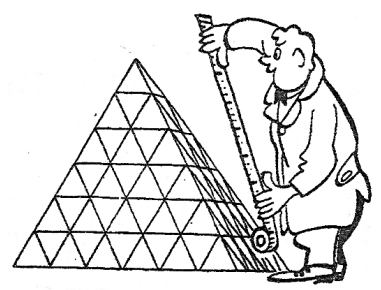
\includegraphics[scale=0.5]{figures/pyramide.png}
\end{center}
Un bureau d’étude a en charge le projet de construction d’une pyramide du style de celle du Louvre (base carrée) de 12 niveaux.
Combien de plaques de verre, toutes identiques et ayant la forme de triangles équilatéraux, sont-elles nécessaires à la réalisation d’un tel ouvrage ?
Un comptage systématique des plaques s’avérant long et fastidieux,
tentons de trouver une méthode de calcul.

\begin{itemize}
\item On notera \(u_{n}\) le nombre de plaques au niveau \(n\), en commançant par le sommet de la pyramide.
Donne les \(6\) premiers termes de la suite \((u_{n})\).
\end{itemize}
\par \setlength{\columnseprule}{0 pt}
          \begin{minipage}[t]{\linewidth}
          \begin{multicols}{3}
\(u_{0}=\dotfill\)

\(u_{1}=\dotfill\)

\(u_{2}=\dotfill\)

\(u_{3}=\dotfill\)

\(u_{4}=\dotfill\)

\(u_{5}=\dotfill\)


\end{multicols}\end{minipage}


Puisque nous ajoutons toujours le même nombre pour passer d’un terme
au suivant, nous sommes en présence d’une suite arithmétique. Le nombre que l’on
ajoute pour passer d’un terme au suivant s’appelle la raison.

\begin{itemize}
\item Comment calcule-t-on \(u_{n}\) à partir de \(n\)? Donne une formule en t'aidant
du dessin de la page suivante:
\dotfill

\dotfill

\begin{center}
\includestandalone[width=\linewidth]{figures/fig5}
\end{center}

\item Utilise la formule que tu viens de trouver pour calculer le nombre
de plaques de verre au \(12\) ème niveau: \(u_{11}=\dotfill\)

\item Représente graphiquement la suite.
\end{itemize}

\begin{center}
\includestandalone[width=0.8\linewidth]{figures/fig6}
\end{center}

Tu constates que les points suivent l'allure d'une \dotfill.

On pourra donc conjecturer qu'une suite arithmétique a aussi cette
représentation. Dans ce cas, on dira qu'une suite arithmétique a une
croissance \dotfill

\begin{itemize}
\item En t'aidant du graphique, calcule le nombre total de plaques de verre nécessaires pour construire la pyramide de \(12\) niveaux:
\end{itemize}


\(S_{12}=\text{ somme des 12 premiers termes }=u_{0}+u_{1}+u_{2}+\cdots+u_{11}=\dotfill\)


\begin{itemize}
\item Peux-tu donner une formule qui permettrait de calculer la somme des
\(n\) premiers termes d'une suite arithmétique?
\end{itemize}


\(S_{n}=\) \dotfill

\dotfill


Pour t'aider, concentre toi sur la suite \((u_{n})\) du nombre de
plaques de verre pour construire la pyramide. Calculons d'une autre
manière \(S_{12}\):
\begin{itemize}
\item calcule
\end{itemize}

\par \setlength{\columnseprule}{0 pt}
          \begin{minipage}[t]{\linewidth}
          \begin{multicols}{3}
\(u_{0}+u_{11}=\dotfill\)

\(u_{1}+u_{10}=\dotfill\)

\(u_{2}+u_{9}=\dotfill\)

\(u_{3}+u_8=\dotfill\)

\(u_{4}+u_7=\dotfill\)

\(u_{5}+u_6=\dotfill\)


\end{multicols}\end{minipage}
\begin{itemize}
\item Que constates-tu?\dotfill

\dotfill
\end{itemize}


\begin{itemize}
\item Déduis-en une formule pour \(S_{12}\) .\dotfill

\dotfill
\item Comment pourrais-tu généraliser?\dotfill

\dotfill
\item Calcule \(S_{16}:\)

\(S_{16}=\) \dotfill
\end{itemize}

\section{Définition}
\label{sec:org2836874}

\begin{definition}
Une suite arithmétique est une suite numérique telle que la
différence entre deux termes consécutifs est constante. Cette
différence est appelée la raison de la suite.
\end{definition}

\begin{remarque}
\begin{itemize}
\item Si la raison est nulle, alors la suite est constante;
\item Le premier terme d'une suite arithmétique sera toujours de rang \(0\).
\end{itemize}
\end{remarque}

\section{Représentation graphique d'une suite.}
\label{sec:org66915cf}
Les suites arithmétiques sont des exemples de modèles de croissance
linéaire: leur représentation suit une droite.

Nous avons déjà pu le constater avec la suite \((C_n)\) des capitaux à
intérêts simples:

\begin{center}
\includestandalone[width=0.6\linewidth]{figures/fig1}
\end{center}

De plus, on peut dire que pour une suite arithmétique de raison \(r\),
\begin{itemize}
\item si \(r>0\), alors la suite est strictement croissante
\item si \(r=0\), alors la suite est constante
\item si \(r<0\), alors la suite est strictement décroissante
\end{itemize}

\section{Génération d'une suite arithmétique}
\label{sec:org320234c}

\subsection{Relation de récurrence et formule explicite}
\label{sec:org31de2e6}

\begin{propriete}
Soit \((u_n)\) une suite arithmétique de raison \(r\) et de premier terme \(a\). Alors

\begin{enumerate}
\item (Relation de récurrence:) \(u_{n+1}=u_{n}+r\), \(u_0=a\).
\item (Formule explicite:) \(u_n=u_0+nr=a+nr\).
\end{enumerate}
\end{propriete}

Par exemple, pour une suite arithmétique de raison 7 et de premier
terme \(-4\),

\begin{itemize}
\item Relation de récurrence: \dotfill

\item Formule explicite:\dotfill

\item \(u_{1000}=\) \dotfill
\end{itemize}

\subsection{Calcul d'un terme à partir d'un autre:}
\label{sec:org5226575}

Calcule le 10e terme d'une suite arithmétique de raison -2 et de 4e
terme 6.

\dotfill

\dotfill

\dotfill

\dotfill

\dotfill

Déduis-en une formule permettant de calculer un terme \(u_n\) à partir
d'un terme \(u_p\) sachant que la suite est arithmétique de raison \(p\):

\begin{propriete}


Soit \((u_n)\) une suite arithmétique de raison \(r\).
Alors, étant donnés \(n,p\in\IN\),

\dotfill
\end{propriete}

\subsection{Calcul de la raison à partir de deux termes de la suites.}
\label{sec:orgdf56e3b}

Calcule la raison d’une suite arithmétique de 21ème terme 120 et de
9ème terme 30

\dotfill

\dotfill

\dotfill

\dotfill

\dotfill

Déduis-en une formule permettant de calculer la raison \(r\) lorsque l’on connait deux termes
\(r_p\) et \(u_n\) :
\begin{propriete}


Soit \((u_n)\) une suite arithmétique de raison \(r\). Alors, étant donnés \(n,p\in\IN\), \(p\neq n\),  \dotfill
\end{propriete}

\section{Caractéristiques des suites arithmétiques}
\label{sec:org2a72294}

\subsection{Variation, limite et convergence}
\label{sec:orgce8967b}
Nous allons distinguer les suites de raison positive de celles de
raison négative.

\begin{center}
\begin{tabular}{|p{3cm}|p{3cm}|p{3cm}|p{3cm}|}
\hline
Raison \(r\) & \(r>0\) & \(r=0\) & \(r<0\)\\[0pt]
\hline
Variation &  &  & \\[0pt]
\hline
\(\lim\limits_{n\to\infty}u_n\) &  &  & \\[0pt]
\hline
Convergence &  &  & \\[0pt]
\hline
\end{tabular}
\end{center}

\subsection{Somme des \(n\) premiers termes}
\label{sec:org04e2fd4}

La somme des \(n\) premiers termes d'une suite est définie comme

\[
S_n=u_0+u_1+u_2+\ldots+u_{n-2}+u_{n-1}.
\]

\uline{\textbf{Attention!}}: dans \(S_n\) on somme jusqu'à l'indice \(n-1\) car on
commence à compter à partir de \(0\)!.

\begin{propriete}
Pour une suite arithmétique, on a
\[
S_n=\dfrac{n}{2}(u_0+u_{n-1}).
\]
\end{propriete}
\begin{proof}
\dotfill

\dotfill

\dotfill

\dotfill

\dotfill

\dotfill

\dotfill

\dotfill

\dotfill

\dotfill

\dotfill

\dotfill

\dotfill
\end{proof}


\section{Exercices}
\label{sec:org6aa25dc}

\begin{exercice}
Parmi les suites suivantes, indique les suites arithmétiques, précise leur raison et donne
leur formule explicite:
\par \setlength{\columnseprule}{0 pt}
          \begin{minipage}[t]{\linewidth}
          \begin{multicols}{2}
\begin{itemize}
\item \((u_n)=(-17;-10;-3;4;11;\ldots)\)
\item \((w_n)=(16;4;-8;-20;\ldots)\)
\item \((y_n)=\left(\dfrac{5}{3};2;\dfrac{7}{3};\dfrac{8}{3};3;\ldots
  \right)\)
\item \((v_n)=(4;8;16;32;\ldots)\)
\item \((x_n)=(1;2;4;5;7;8;\ldots)\)
\end{itemize}


\end{multicols}\end{minipage}
\end{exercice}

\begin{exercice}
Une suite arithmétique \((x_n)\) a pour premier terme \(x_1=-4\) et
pour raison \(r=3\). Calcule ses 5 premiers termes, donne son sens de
variation, donne sa formule explicite et calcule son 100ème
terme. Simplifie tes résultats au maximum.
\end{exercice}

\begin{exercice}
Soit la suite définie par la relation \(u_{n+1}=u_n-5\),
\(u_0=-2\). Quelle est la raison, la variation et la limite de cette suite?
\end{exercice}

\begin{exercice}
\((t_0;t_1;t_2;t_3;\ldots;t_n;\ldots)\) sont les termes d'une suite
arithmétique, dont la raison est \(r\).

\begin{center}
\begin{tabular}{|p{6cm}|p{6cm}|}
\hline
On te donne: & Trouve:\\[0pt]
\hline
\(t_3=6\), \(r=1/2\) & \(t_1,t_9,t_{20}\)\\[0pt]
\hline
\(t_2\), \(r=-2\) & \(t_{13}\), \(t_{22}\)\\[0pt]
\hline
\(t_3=1\), \(t_{10}=15\) & \(t_1,t_{29}\)\\[0pt]
\hline
\(t_0=10\), \(t_{10}=-17\) & \(S_{10}\)\\[0pt]
\hline
\(t_0=-3\), \(r=4\) & \(S_7\)\\[0pt]
\hline
\(t_0\), \(S_5=37,5\) & \(t_5\), \(r\)\\[0pt]
\hline
\(t_0\), \(t_4=11\) & \(S_{35}\)\\[0pt]
\hline
\end{tabular}
\end{center}
\end{exercice}

\begin{exercice}
Dans la suite arithmétique \((u_n)=(1;7;13;\ldots)\),
\begin{itemize}
\item quel est le rang du terme valant 295?
\item que vaut \(1+7+13+\cdots+295\)?
\end{itemize}
\end{exercice}

\begin{exercice}
Calcule les sommes suivantes:
\begin{enumerate}
\item \(-5-2+1+4+\cdots+52\)
\item \(1-4-9-\cdots-504\)
\end{enumerate}
\end{exercice}

\begin{exercice}
Dans une suite arithmétique, la somme des 10 premiers termes est 245
et la différence des extrêmes \(u_0-u_{10}\)  est 45. Donne une formule
explicite de cette suite.
\end{exercice}

\begin{exercice}
Au mois de janvier 2015, Vincent a économisé 12,50\texteuro{} ; au mois de
février, il a économisé 1,20\texteuro{} de plus qu’en janvier ; au mois de
mars, il a économisé 1,20\texteuro{} de plus qu’en février, etc. Il
économise ainsi chaque mois 1,20\texteuro{} de plus que le mois précédent. On note
\(u_0\) , l’économie de janvier 2015, \(u_1\) , l’économie de février
2015, \(u_2\) , l’économie de mars 2015 et ainsi de suite

\begin{enumerate}
\item Comment noter l’économie réalisée en décembre 2016 ?
\item Calcule \(u_1\) , \(u_2\) , \(u_3\) , \(u_4\) .
\item Exprime \(u_n\) en fonction de \(n\).
\item Quelle somme Vincent va-t-il économiser en décembre 2016 ?
\item Quelle somme totale Vincent aura-t-il économisée de janvier 2015 à
décembre 2016 ?
\end{enumerate}
\end{exercice}

\begin{exercice}
Une personne achète un article et désire le rembourser
mensuellement. Le premier mois, il paie 600\texteuro{} et les mensualités
suivantes augmentent de 10\texteuro{} chaque mois. Quelle  est la 7ème
mensualité ? Quel est le prix de l’article sachant qu’il y a 15
mensualités ?
\end{exercice}

\begin{exercice}
Un charpentier désire construire une échelle avec 9 échelons dont la longueur
diminue de manière régulière de 45 cm à la base à 33 cm au sommet

\begin{itemize}
\item Détermine la longueur des 7 échelons intermédiaires.
\item Détermine la longueur totale de bois nécessaire pour fabriquer les 9 échelons.
\end{itemize}
\end{exercice}

\begin{exercice}
Un jardinier doit déposer une brouette de terreau au pied de chacun des 30 arbres
formant un côté d'une allée de son jardin. Les arbres sont à 6 mètres de distance les
uns des autres, et le tas de terreau est à 10 mètres en avant du 1er arbre du même
côté de l'allée.
Combien de km, le jardinier aura-t-il parcouru après avoir achevé son travail et ramené
la brouette près du tas de terreau sachant qu’entre 2 arbres, il revient
systématiquement au tas de terreau ?
\end{exercice}

\chapter{Suites géométriques}
\label{sec:orge17a8ab}
\section{Pliage d'une feuille de papier}
\label{sec:org5a3b62c}

Une feuille de papier a une épaisseur de \(0,1\) mm. On note \(t_{0}\) cette épaisseur.

On plie ensuite cette feuille une première fois en deux. On note \(t_{1}\) l'épaisseur de la feuille après un pliage.

On plie à nouveau la feuille en deux. On note \(t_{2}\) l'épaisseur
après ce deuxième pliage et ainsi de suite.

\begin{itemize}
\item Complète le tableau ci-dessous.

\begin{center}
\begin{tabular}{|l|p{1cm}|p{1cm}|p{1cm}|p{1cm}|p{1cm}|p{1cm}|p{1cm}|}
\hline
Nombre de pliages & 0 & 1 & 2 & 3 & 4 & 5 & 5\\[0pt]
\hline
Épaisseur de la feuille &  &  &  &  &  &  & \\[0pt]
\hline
\end{tabular}
\end{center}

Qu'observes-tu?\dotfill

\dotfill

\item Quelle est l'épaisseur:
\begin{itemize}
\item après 10 pliages:\dotfill
\item après 15 pliages: \dotfill

\item après \(n\) pliages:\dotfill
\end{itemize}

\begin{center}
\includestandalone[width=0.8\linewidth]{figures/fig8}
\end{center}
\item Voici la représentation des premiers termes de la suite.

\begin{center}
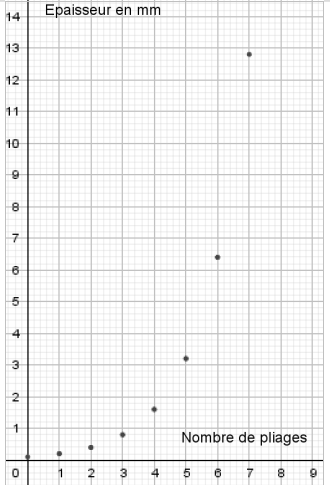
\includegraphics[width=0.5\linewidth]{figures/fig8.png}
\end{center}
\end{itemize}
Comme tu peux le voir, cette suite croît extrêmement rapidement.

Si c’était possible de le faire, après 20 pliages, on obtiendrait une épaisseur de l’ordre de 100 m.
En effet, \(t_{20}=\) \dotfill

Après 51 pliages, l’épaisseur de la feuille aurait dépassé la distance
de la terre au soleil !

\section{Définition}
\label{sec:org11de80d}

\begin{definition}
Une suite géométrique est une suite numérique telle que le rapport
entre deux termes consécutifs est constante (\textbf{non nulle!}). Ce
rapport est appelé la raison de la suite.
\end{definition}

\begin{remarque}
\begin{itemize}
\item Si la raison vaut \(1\) , alors la suite est constante;
\item Le premier terme d'une suite géométrique sera toujours de rang \(0\).
\end{itemize}
\end{remarque}

\section{Représentation graphique d'une suite.}
\label{sec:org510f203}
Les suites géométriques sont des exemples de modèles de croissance
exponentielle: leur représentation suit une courbe dont la croissance
est rapide.

Nous avons déjà pu le constater avec la suite \((C_n)\) des capitaux à
intérêts composés:

\begin{center}
\includestandalone[width=0.6\linewidth]{figures/fig2}
\end{center}

Nous verrons plus tard que les suites géométriques peuvent avoir des
comportements forts différents en fonction de la raison \textbf{et} du
premier terme.
\section{Génération d'une suite géométrique}
\label{sec:orge9783fa}

\subsection{Relation de récurrence et formule explicite}
\label{sec:org68af152}

\begin{propriete}
Soit \((u_n)\) une suite géométrique de raison \(r\) et de premier terme \(a\). Alors

\begin{enumerate}
\item (Relation de récurrence:) \(u_{n+1}=u_{n}\cdot r\), \(u_0=a\).
\item (Formule explicite:) \(u_n=u_0\cdot r^n=a\cdot r^n\).
\end{enumerate}
\end{propriete}

Par exemple, pour une suite géométrique de raison 7 et de premier
terme \(-4\),

\begin{itemize}
\item Relation de récurrence: \dotfill

\item Formule explicite:\dotfill

\item \(u_{5}=\) \dotfill
\end{itemize}

\subsection{Calcul d'un terme à partir d'un autre:}
\label{sec:orgc74fcdc}

Calcule le 10e terme d'une suite arithmétique de raison -2 et de 4e
terme 6.

\dotfill

\dotfill

\dotfill

\dotfill

\dotfill

Déduis-en une formule permettant de calculer un terme \(u_n\) à partir
d'un terme \(u_p\) sachant que la suite est géométrique de raison \(p\):

\begin{propriete}


Soit \((u_n)\) une suite arithmétique de raison \(r\).
Alors, étant donnés \(n,p\in\IN\),

\dotfill
\end{propriete}

\subsection{Calcul de la raison à partir de deux termes de la suites.}
\label{sec:org43ddc16}

Calcule la raison des suites géométriques suivantes:

\begin{itemize}
\item \(u_2=6\) et \(u_5=20,25\)
\end{itemize}
\dotfill

\dotfill

\dotfill

\begin{itemize}
\item \(u_2=6\) et \(u_5=-20,25\)
\end{itemize}
\dotfill

\dotfill

\dotfill

\begin{itemize}
\item \(u_2=6\) et \(u_6=30,375\)
\end{itemize}
\dotfill

\dotfill

\dotfill

Déduis-en une formule permettant de calculer la raison \(r\) lorsque l’on connait deux termes
\(r_p\) et \(u_n\) :
\begin{propriete}


Soit \((u_n)\) une suite arithmétique de raison \(r\). Alors, étant donnés
\(n,p\in\IN\), \(p\neq n\),

\begin{itemize}
\item si \(n-p\) est pair, alors \dotfill

\item si \(n-p\) est impair, alors \dotfill
\end{itemize}
\end{propriete}

\section{Caractéristiques des suites arithmétiques}
\label{sec:orgb891dd6}

\subsection{Variation, limite et convergence}
\label{sec:orgd93c37e}
Nous allons distinguer les suites de raison positive de celles de
raison négative. De plus, le signe du premier terme sera déterminant.

Voici quelques suites, toutes géométriques.

\begin{center}
\includestandalone[width=1\linewidth]{figures/fig9}
\end{center}

\begin{center}
\includestandalone[width=1\linewidth]{figures/fig10}
\end{center}

\begin{center}
\begin{tabular}{|p{1.2cm}|p{2.9cm}|p{2.9cm}|p{2.9cm}|p{2.9cm}|p{2.9cm}|}
\hline
 & \(r\le-1\) & \(-1<0<1\) & \(0<r<1\) & \(r=1\) & \(r>1\)\\[0pt]
\hline
\(u_0>0\) & \(\lim\limits_{n\to\infty}u_n\ldots\ldots\) & \(\lim\limits_{n\to\infty}u_n\ldots\ldots\) & \(\lim\limits_{n\to\infty}u_n\ldots\ldots\) & \(\lim\limits_{n\to\infty}u_n\ldots\ldots\) & \(\lim\limits_{n\to\infty}u_n\ldots\ldots\)\\[0pt]
\hline
\(u_0<0\) & \(\lim\limits_{n\to\infty}u_n\ldots\ldots\) & \(\lim\limits_{n\to\infty}u_n\ldots\ldots\) & \(\lim\limits_{n\to\infty}u_n\ldots\ldots\) & \(\lim\limits_{n\to\infty}u_n\ldots\ldots\) & \(\lim\limits_{n\to\infty}u_n\ldots\ldots\)\\[0pt]
\hline
\end{tabular}
\end{center}

\subsection{Somme des \(n\) premiers termes}
\label{sec:orgb6e1239}

La somme des \(n\) premiers termes d'une suite est définie comme

\[
S_n=u_0+u_1+u_2+\ldots+u_{n-2}+u_{n-1}.
\]

\uline{\textbf{Attention!}}: dans \(S_n\) on somme jusqu'à l'indice \(n-1\) car on
commence à compter à partir de \(0\)!.

\begin{propriete}
Pour une suite géométrique \textbf{de raison} \(r\neq 1\), on a
\[
S_n=u_0\frac{r^n-1}{r-1}.
\]
\end{propriete}
\begin{proof}
\dotfill

\dotfill

\dotfill

\dotfill

\dotfill

\dotfill

\dotfill

\dotfill

\dotfill

\dotfill

\dotfill

\dotfill

\dotfill
\end{proof}


\section{Exercices}
\label{sec:orgc44144d}
\begin{exercice}
Parmi les suites suivantes, indique les suites géométriques, précise leur raison et
donne leur formule explicite.

\par \setlength{\columnseprule}{0 pt}
          \begin{minipage}[t]{\linewidth}
          \begin{multicols}{2}
\begin{itemize}
\item \((u_n)=(1;0.1;0.01;0.001;\ldots)\)
\item \((v_n)=(3;5;7;9;11;\ldots)\)
\item \((w_n)=(7;7,5;43,75;109,375;\ldots)\)
\item \((z_n)=\left(\dfrac{1}{3};\dfrac{2}{9};\dfrac{4}{27};\dfrac{8}{81};\ldots\right)\)
\end{itemize}


\end{multicols}\end{minipage}
\end{exercice}
\uline{\textbf{Les suites des exercices suivants sont des suites géométriques.}}
\begin{exercice}
Dans chaque cas, calcule \(u_1,u_2,u_3,u_4\) . Donne leur formule
explicite et calcule \(u_9\) et \(S_{10}\).
Précise la variation et la convergence de la suite.
\begin{itemize}
\item \(u_0=-7\) et \(r=3\)
\item \(u_0=128\) et \(r=\dfrac{1}{2}\)
\end{itemize}
\end{exercice}

\begin{exercice}
Dans chaque cas, calcule \(u_0,u_6\) et \(S_7\) .
Précise la variation et la convergence de la suite.
\begin{itemize}
\item \(u_4=512\) et \(r=2\)
\item \(u_2=\dfrac{9}{4}\) et \(r=\dfrac{1}{3}\)
\end{itemize}
\end{exercice}

\begin{exercice}
Dans chaque cas, calcule \(u_0\) et la raison.

\begin{itemize}
\item \(u_5=567\) et \(u_6=15309\)
\item \(u_5=7012758,654\) et \(u_1=5350000\)
\end{itemize}
\end{exercice}

\begin{exercice}
Dans chaque cas, calcule le dernier terme de la somme, ensuite calcule
la somme des suites géométriques suivantes :

\begin{itemize}
\item \(S_{12}=8+16+32+\cdots\)

\item \(S_{11}=\dfrac{1}{2}+\dfrac{1}{4}+\dfrac{1}{8}+\cdots\)
\end{itemize}
\end{exercice}

\begin{exercice}
Calcule \(3+6+12+\ldots+1536\).
\end{exercice}

\begin{exercice}
Calcul \(S_{12}\) si \(u_3=281,04\) et \(u_8=341,93\).
\end{exercice}

\begin{exercice}
Le premier terme d’une suite géométrique est −21 et le troisième est
−189. Quelle est la raison ?
\end{exercice}

\begin{exercice}
Sachant que \((u_n)\) est une suite géométrique, que \(u_3\) vaut 24 et
que \(u_{11}\) vaut 6144, calcule \(u_0\).
\end{exercice}

\begin{exercice}
Insère 5 termes entre 2 et 31250 pour former une suite géométrique.
\end{exercice}

\begin{exercice}
Le prix initial d’un sac est de 165 euros. Celui-ci a subi 4 rabais
successifs de 5\% à l’occasion des soldes.
\begin{itemize}
\item Calcule son prix après chaque rabais.
\item Quelle est la nature de la suite formée par ces différents prix ?
\item Quel est le pourcentage total de diminution ?
\end{itemize}
\end{exercice}

\begin{exercice}
Le prix de vente d’une brochure augmente de 3\% chaque fin d’année. Quel sera son
prix à la fin de la 10ème année sachant que son prix initial est de 4,5\texteuro{} ?
\end{exercice}

\begin{exercice}
La légende veut que l’inventeur du jeu d’échecs, remercié par le roi de Perse, ait
demandé en récompense, un grain de blé pour la première case de l’échiquier, deux
grains pour la deuxième, quatre pour la troisième et ainsi de suite en doublant, chaque
fois, le nombre de grains jusqu’à la 64ème case. Le roi trouva cette demande bien
modeste ! Cette demande était-elle réaliste ?

\emph{Indication : la production mondiale de blé en 2012-2013 s’élevait à 713 millions de
tonnes et 100 grains de blé pèsent environ 5g}
\end{exercice}

\begin{exercice}
On construit une spirale dont chaque demi-cercle a un rayon double de celui du demi-
cercle précédent. Quelle est la longueur de cette spirale lorsqu’elle est formée de 9 demi-
cercles sachant que le rayon du premier demi-cercle mesure 3cm ?
\end{exercice}

\begin{exercice}
Une balle est lancée d’une hauteur de 2 m. A chaque fois qu’elle touche le sol, elle
rebondit jusqu’à 75\% de sa hauteur précédente.
\begin{itemize}
\item Quelle hauteur atteint la balle après le troisième rebond ?
\item Quelle hauteur atteint la balle après le 𝑛ième rebond ?
\item Combien de fois la balle doit-elle rebondir avant que la hauteur
soit inférieure à 15 cm ?
\end{itemize}
\end{exercice}
\end{document}
